\chapter{Safety}

To explore Mars it is necessary to take the safety of the robot into account. The Martian environment has to be taken into consideration, to keep the robot safe.
As described in chapter \ref{ch:environmentOnMars} the temperature ranges differs a lot, which is why a robot on Mars needs to be able to handle such range of temperatures. Additionally, it is also important to take into consideration, that there are dust storms on Mars, see figure \ref{fig:Duststorm }. The strongest wind during dust storms is 97 km/h. A robot in this environment has to have a low center of mass to handle these strong winds\cite{AspectsWeather} \cite{AspectsTemperature}.

\begin{figure}[h]
    \centering
    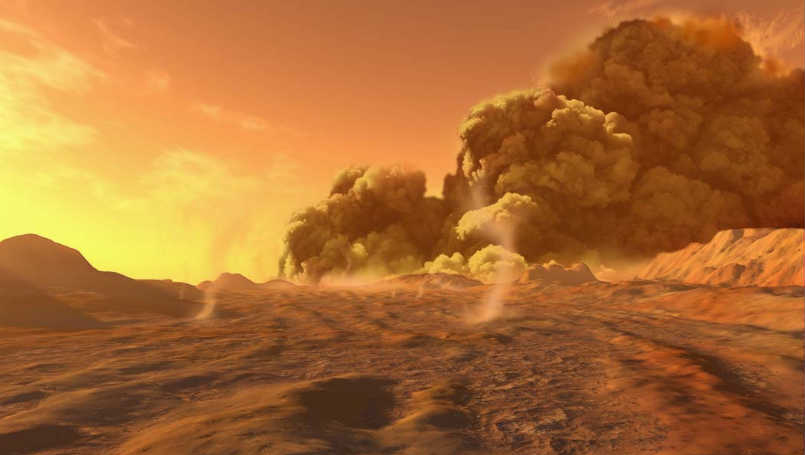
\includegraphics[width=.7\textwidth]{figures/dust-storm-on-mars2.jpg}
    \caption{Artist impression of dust storm on Mars \cite{Duststorm}} 
    \label{fig:Duststorm } 
\end{figure}

For the safety of the Martian environment, a robot on Mars has to keep its distance to water, ice, and other geology definitions due to specific regulations, as explained in chapter \ref{ch:Spacelaw}. In addition to this, INEX has to be able to detect all the definitions and respond appropriately\cite{AspectsWeather}.


%The atmosphere of Mars consists of 95\% CO$_2$. During the winter, the atmosphere is cold enough to condense CO$_2$ into CO$_2$-ice caps.

%extra

%\newpage

%\section{Social Aspects}
%\begin{figure}[h]
    %\centering
    %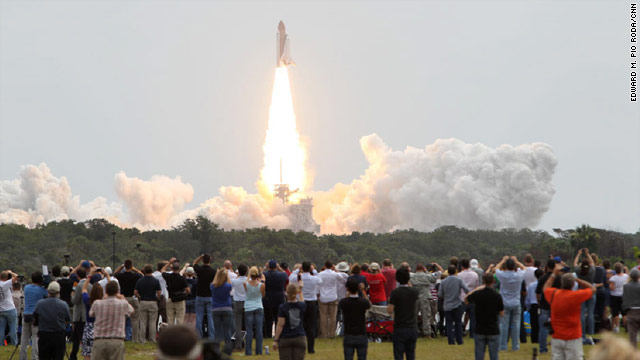
\includegraphics[width=\textwidth]{figures/1356.jpg}
    %\caption{ALWAYS REMEMBER CAPTION UNDER PICTURES (edit the label and a picture if there is a %picture you HAVE to refer to it in the text, which you do with the label) AND remember cite %if it's not your own picture/illustration}
    %\label{fig:randomfiglabel} %Make your own label so you can refer to it in the text. If you have trouble with this ask Natalie
%\end{figure}%\todo{Caption and label in picture needed}

%Nowadays any technological progress that is able to make it to the mainstream media
%has a strong impact on the general thinking of society.
%Exploring space and being able to go beyond Earth's orbit, has been one of the goals that has formed modern mentality of human society in a way that once, being able to fly did.
%Each question we find the answer for, becomes a doorway for more questions and creates the ground for means of answering them.
%The one planet that attracts the most attention and curiosity, is our closest neighbor Mars.
%Raising the chances for a project to get funded goes hand in hand with how much influence it can create on the targeted area and that's the fact.\\
%Considering the Mars missions and the changes in perspectives our new understandings of this planet could bring about, we could always expect positive social reinforcement and look at society as one of the main sources of feedback.%\todo( find or add some source )
\\


